\documentclass{beamer}
% Copyright 2008 by Daina Chiba <daina.chiba@gmail.com>
%
% This file can be redistributed and/or modified under
% the terms of the GNU Public License, version 2.

% Example presentation template file for beamerthemeRice version 0.02 (2008/11/22)

%===============================================================%
\mode<presentation> %use <handout> for handout mode
% \mode<handout> %use <handout> for handout mode
{
\usetheme[compress, nologo, numbers]{Rice}
%\usetheme[ricet, smoothb]{Rice}
%\usetheme[riceb, minimal]{Rice}
	% [ricet]		show the \Large "RICE" word mark at the top-right
	% [ricetm]		show the \large "RICE" word mark at the top-right
	% [ricets]		show the \small "RICE" word mark at the top-right
	% [riceb]		show the "RICE" word mark at the bottom-left
	% [compress]	show only the current section / subsection in the top navigation area.
	%			recommended if you have more than three subsections in at least one section
	% [minimal]	hide top navigation
	% [numbers]	show page numbers at the bottom-right
	% [noshadow]	remove shadow
	% [nologo]	remove Rice logo from the title page
	% [ricegray]	use ricegray instead of riceblue
	% [bgricegray]	use ricegray as background color
	% [bggray]	use light gray as background color
	% [smoothb]	top navigation with balls
\usefonttheme[onlymath]{serif}
	% \useoutertheme{infolines}
\setbeamercovered{transparent}
}
% In case you want to use other themes with riceblue...
%\usetheme{Frankfurt}
% AnnArbor, Antibes, Berlin, Berkeley, Bergen, Boadilla, boxes, CambridgeUS, Copenhagen
% Darmstadt, Dresden, Frankfurt
%\usecolortheme{riceowl}

\usepackage[english]{babel}
% \beamerdefaultoverlayspecification{<+->}

\usepackage{mathptmx}
\usepackage{helvet}
\usepackage{courier}
% \usepackage{arev}
\usepackage[T1]{fontenc}
\usepackage{trajan}
\usepackage{minted}
\usepackage{hyperref}
\usepackage{listings}

\lstset{basicstyle=\ttfamily,
  showstringspaces=false,
  commentstyle=\color{magenta},
  keywordstyle=\color{blue},
  frame=single,
  language=bash
}
%===============================================================%

\title[GitHub Tutorials]
{GitHub Tutorials}

\subtitle
% {for 2020 ASME-CIE Hackathon: Identifying, Extracting, Analyzing Value from Large Unstructured Data Sets in Mechanical Engineering}
{for 2020 ASME-IMECE Hackathon: Identifying, Extracting, Analyzing Value from Large Unstructured Data Sets in Mechanical Engineering}

\author[Anh Tran]{Anh Tran}
\institute
{
 Optimization and Uncertainty Quantification Department \\
 Computer Science Research Institute \\
 Sandia National Laboratories \\
}

% \date[11.22.2008]{Nov. 22, 2008}
\date{\today}

\subject{Beamer}


\begin{document}

% Comment out the following to remove the header & footer from the title page
% \thispagestyle{empty} 

\begin{frame}
 \titlepage
\end{frame}

\begin{frame}<beamer>
 \frametitle{Outline}
 \tableofcontents
\end{frame}

\section{Introduction}

\begin{frame}
\frametitle{What is GitHub?}

\begin{block}{Software development}
Git is the free and open source distributed version control system that's responsible for everything GitHub related that happens locally on your computer. 
\end{block}



\begin{itemize}
\item \href{https://education.github.com/git-cheat-sheet-education.pdf}{\underline{This}} cheat sheet is your friend,
\item but \href{https://guides.github.com/}{\underline{other official guides}} are also available


\end{itemize}

\end{frame}


\section{Hello World}

\begin{frame}
\frametitle{Hello World}

\begin{itemize}
\item go to \href{https://www.github.com}{\underline{https://www.github.com}}
\item create an account (it's free!)
\item create a new repository (``repo'')
\begin{itemize}
\item choose your favorite license for your implementation (you own your codes!)
\item write a README.md
\end{itemize}
\item invite others to join your GitHub repo
\end{itemize}

\end{frame}

\section{Setup}

\begin{frame}[fragile]
\frametitle{GitHub Setup}


\begin{itemize}

\item config to $\sim$/.config

\tiny
\begin{verbatim}
git config --global user.name "FirstName LastName"
git config --global user.email "a@b.com"
git config --global color.ui auto
git config --global core.editor "nano" # or your fav editor
\end{verbatim}
\normalsize

\item (optional) create a long-term key to your own device (i.e. if somebody uses your laptop then they can get to your GitHub repo WITHOUT logins)

\tiny
\begin{verbatim}
ssh-keygen -t rsa -b 4096 -C "a@b.com"
# when prompt, type id_rsaGitHub
# will generate id_rsaGitHub and id_rsaGitHub.pub
eval `ssh-agent -s` # start an ssh agent
ssh-add ~/.ssh/id_rsaGitHub # add ssh-key to ~/.ssh/config
# then add ssh public key into Git account through web interface
ssh -vT git@github.com

# expect a message like this
Hi XXX! You've successfully authenticated, but GitHub does not provide shell access.
\end{verbatim}
\normalsize

\end{itemize}

\end{frame}

\section{Code Development}

\begin{frame}[fragile]
\frametitle{Git in action}

\begin{itemize}

\item clone
\tiny
\begin{verbatim}
git clone https://github.com/pytorch/pytorch.git # https
# git clone git@github.com:pytorch/pytorch.git # ssh - SSH required 
# you can also switch mode in ./git/config in the local GitHub repo
\end{verbatim}
\normalsize



\item typical workflow (this is what you will use the most)
\tiny
\begin{verbatim}
git add # be specific, e.g. git add testABC.py
# git add * # this is ok, but beware of your colleagues' concurrent work
# NEVER USE: git add * -f

git commit # or git commit -m "write some notes", git commit --amend
git pull --rebase # git fetch # optional: only if there are conflicts

git push # or git push origin master
# or git stash: https://git-scm.com/docs/git-stash
\end{verbatim}
\normalsize

\item read logs from your teammates
\tiny
\begin{verbatim}
git log
\end{verbatim}
\normalsize

\item remove, copy, move
\tiny
\begin{verbatim}
git rm file.txt
git mv file.txt test/
\end{verbatim}
\normalsize

\item see what have been changed
\tiny
\begin{verbatim}
git diff 
# or 
git diff SHA1 SHA2
\end{verbatim}
\normalsize


\item check status
\tiny
\begin{verbatim}
git status
\end{verbatim}
\normalsize


\end{itemize}
\end{frame}






\begin{frame}[fragile]
\frametitle{Git in action (advanced)}

\begin{itemize}

\item reset to previous version (advanced)
\tiny
\begin{verbatim}
git reset --hard <SHA> # e.g. commit a5fdab97d911414660683c89b6cecd965b55ce16
\end{verbatim}
\normalsize

\item create a branch
\tiny
\begin{verbatim}
git branch my_debug_branch
git checkout my_debug_branch

git checkout master
git merge my_debug_branch

# git branch -v
# git branch -list
\end{verbatim}
\normalsize

\item other helpful sources: \href{https://github.com/allenwhm/git-in-action#what-is-git}{\underline{here}}

\end{itemize}
\end{frame}













\section{README.md}

\begin{frame}[fragile]
\frametitle{README.md}

\begin{itemize}
\item Pandoc/markdown style; official guide \href{https://guides.github.com/features/mastering-markdown/}{\underline{here}}

\item text
\tiny
\begin{verbatim}
It's very easy to make some words **bold** 
and other words *italic* with Markdown. 
You can even [link to Google!](http://google.com)
\end{verbatim}
\normalsize

\item headers
\tiny
\begin{verbatim}
# This is an <h1> tag
## This is an <h2> tag
###### This is an <h6> tag
\end{verbatim}
\normalsize

\item emphasis
\tiny
\begin{verbatim}
*This text will be italic*
_This will also be italic_
**This text will be bold**
__This will also be bold__
_You **can** combine them_
\end{verbatim}
\normalsize

\item strikethrough
\tiny
\begin{verbatim}
~~this~~
\end{verbatim}
\normalsize

\end{itemize}

\end{frame}







\begin{frame}[fragile]
\frametitle{README.md}

\begin{itemize}

\item list: unordered
\tiny
\begin{verbatim}
* Item 1
* Item 2
  * Item 2a
  * Item 2b
\end{verbatim}
\normalsize

\item list: ordered
\tiny
\begin{verbatim}
1. Item 1
1. Item 2
1. Item 3
   1. Item 3a
   1. Item 3b
\end{verbatim}
\normalsize


\item images
\tiny
\begin{verbatim}
![GitHub Logo](/images/logo.png)
Format: ![Alt Text](url)
\end{verbatim}
\normalsize

\item hyperlink
\tiny
\begin{verbatim}
http://github.com - automatic!
[GitHub](http://github.com)
\end{verbatim}
\normalsize

\item inline code
\tiny
\begin{verbatim}
I think you should use an
`<addr>` element here instead.
\end{verbatim}
\normalsize

\end{itemize}

\end{frame}










\begin{frame}[fragile]
\frametitle{README.md}

\begin{itemize}

\item GitHub flavored markdown
\tiny
\begin{verbatim}
```python
def foo():
    if not bar:
        return True
```


```matlab
function y = foo(x)
  y = x
end
```
\end{verbatim}
\normalsize


\end{itemize}

\end{frame}







\section{GitHub Desktop}

\begin{frame}[fragile]
\frametitle{GitHub Desktop (GUI): \href{https://desktop.github.com/}{https://desktop.github.com/}}
\begin{figure}[!htbp]
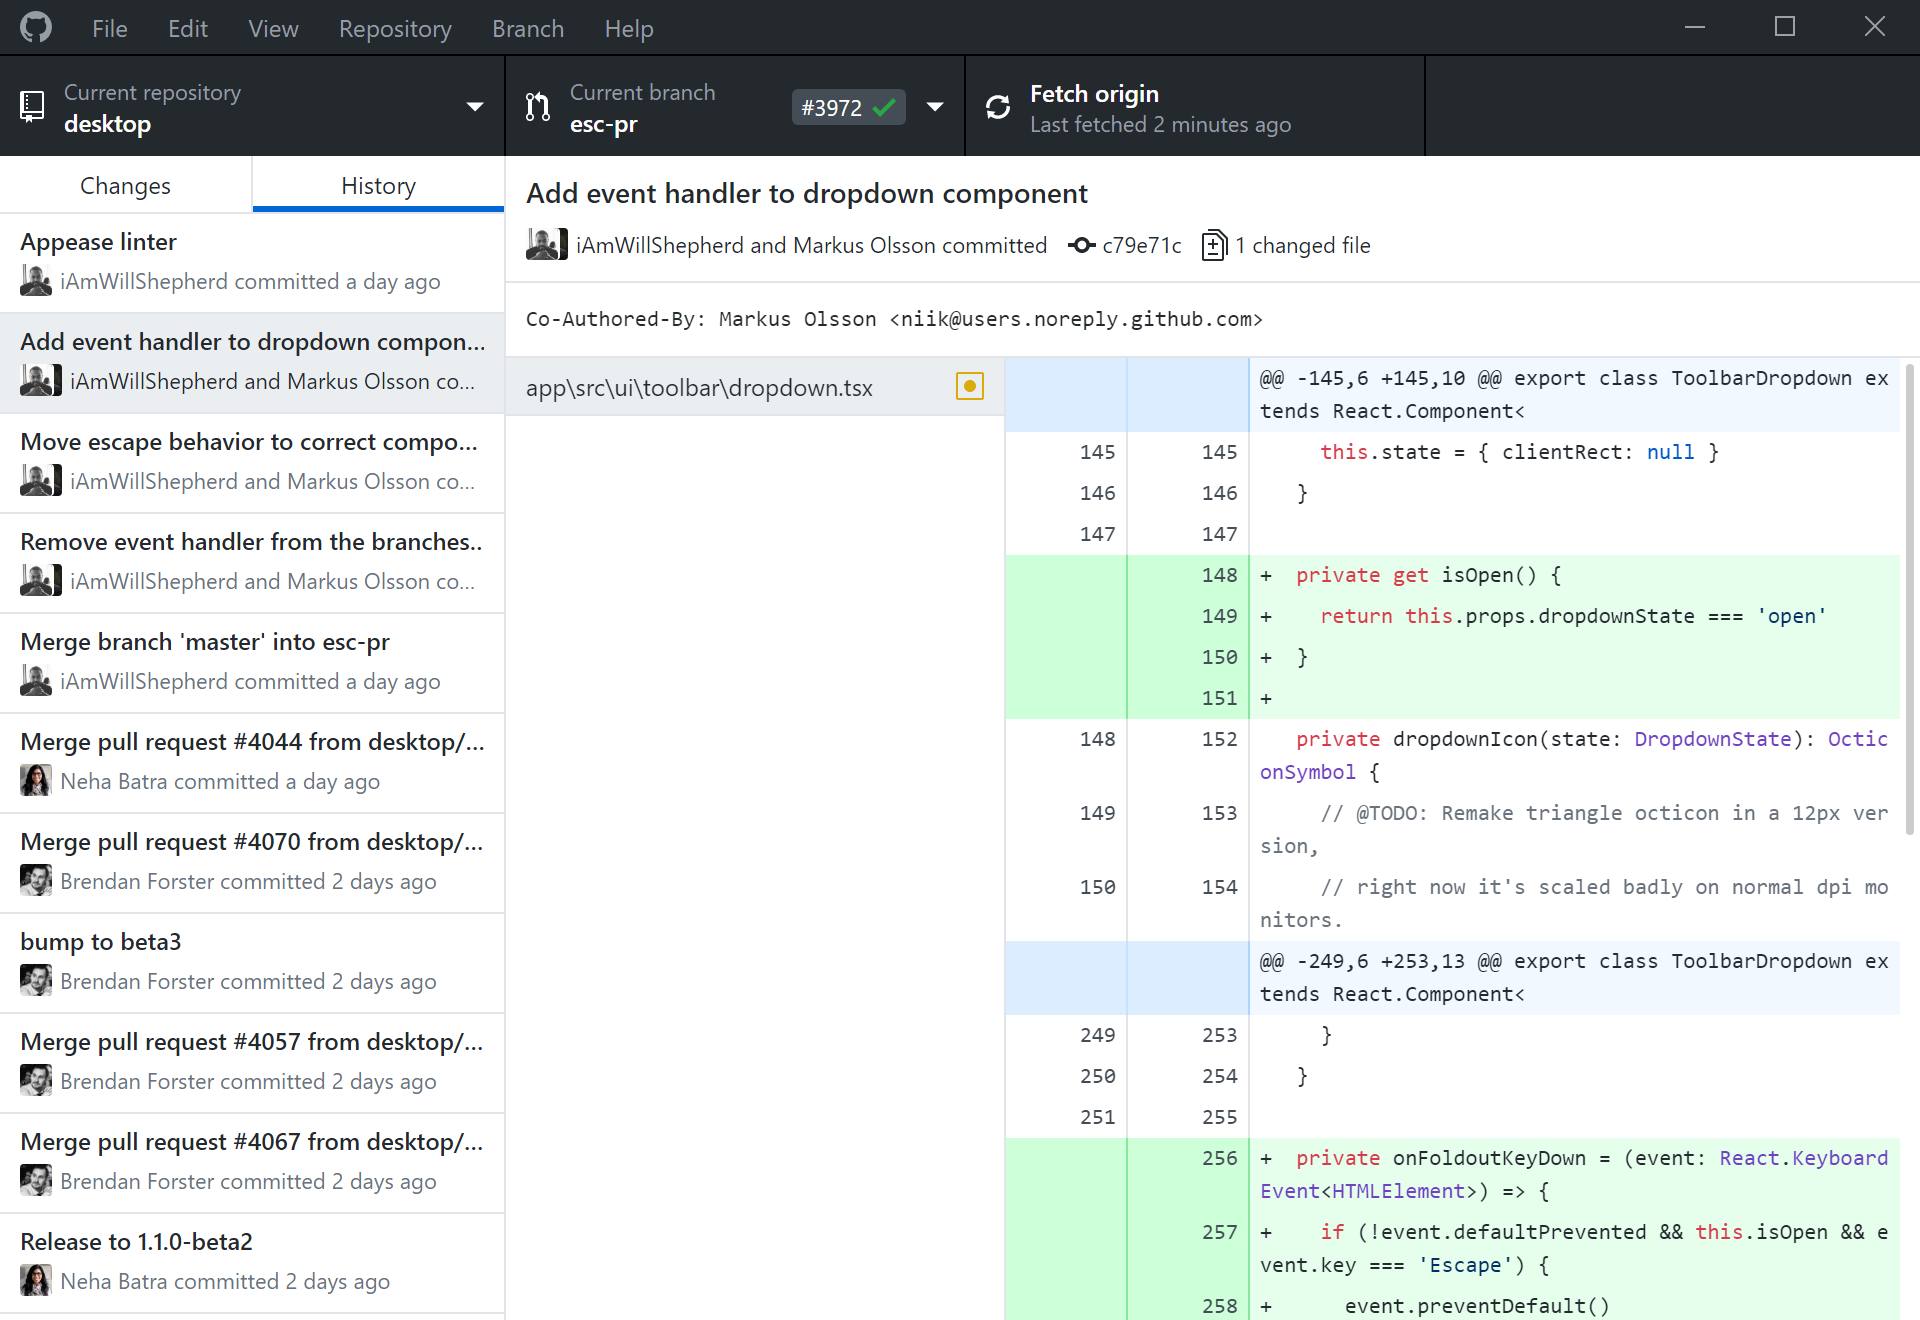
\includegraphics[width=\textwidth,keepaspectratio]{figs/github-desktop-screenshot-windows.png}
\caption{GitHub Desktop}
\end{figure}
\end{frame}





\begin{frame}[fragile]
\frametitle{GitHub Desktop (GUI): \href{https://desktop.github.com/}{https://desktop.github.com/}}
\begin{itemize}
\item official docs: \href{https://docs.github.com/en/free-pro-team@latest/desktop}{https://docs.github.com/en/free-pro-team@latest/desktop}
\item install and configure GitHub Desktop: \href{https://docs.github.com/en/free-pro-team@latest/desktop/installing-and-configuring-github-desktop}{https://docs.github.com/en/free-pro-team@latest/desktop/installing-and-configuring-github-desktop}
\item contributing and collaborating using GitHub Desktop: \href{https://docs.github.com/en/free-pro-team@latest/desktop/contributing-and-collaborating-using-github-desktop}{https://docs.github.com/en/free-pro-team@latest/desktop/contributing-and-collaborating-using-github-desktop}
\end{itemize}
\end{frame}




\end{document}
